\documentclass[12pt,a4paper]{article}
\usepackage{ctex,hyperref}% 输出汉字
\usepackage{times}% 英文使用Times New Roman
\usepackage{amsmath}
\usepackage{hyperref}
\usepackage{bm}
\usepackage{listings}
\usepackage{graphicx}
\usepackage{amsmath}
\usepackage{graphicx}
\usepackage{threeparttable}
\usepackage{float}
\usepackage{amssymb}
\usepackage{caption}
\usepackage{graphicx, subfig}
\usepackage{cite}
\usepackage{titlesec}
\usepackage{geometry}
\usepackage{titlesec}
\usepackage{appendix}
\usepackage{listings}
\usepackage{color}
\usepackage{multirow}
\usepackage{amsmath}
\usepackage[table,xcdraw]{xcolor}
\usepackage{setspace}

\usepackage{fancyhdr}%页眉页脚设定

\usepackage{array}
\usepackage{bookmark}
\usepackage{CJKutf8}
\usepackage{enumerate}
\definecolor{dkgreen}{rgb}{0,0.6,0}
\definecolor{gray}{rgb}{0.5,0.5,0.5}
\definecolor{mauve}{rgb}{0.58,0,0.82}
\lstset
{frame=tb,
 language=Python,
 aboveskip=3mm,
 belowskip=3mm,
 showstringspaces=false,
 columns=flexible,
 basicstyle={\small\ttfamily},
 numbers=left,%设置行号位置none不显示行号
 %numberstyle=\tiny\courier, %设置行号大小
 numberstyle=\tiny\color{gray},
 keywordstyle=\color{blue},
 commentstyle=\color{dkgreen},
 stringstyle=\color{mauve},
 breaklines=true,
 breakatwhitespace=true,
 escapeinside=``,%逃逸字符(1左面的键),用于显示中文例如在代码中`中文...`
 tabsize=4,
 extendedchars=false %解决代码跨页时,章节标题,页眉等汉字不显示的问题
}

\setlength{\parindent}{2em}
\date{\today}

\title{前景分割}
\author{fm}
\begin{document}
\begin{CJK}{UTF8}{gbsn}
\begin{sloppypar}
\maketitle
\section{低层视觉及传统方法:前景分割}
\subsection{简介}
前景分割(Foreground Segmentation)是图像处理和计算机视觉中的一个重要任务,旨在从图像中
分离出感兴趣的前景物体。其目标是将图像中的前景物体与背景进行区分,以便进一步的分析和处理。

传统的图像分割方法依赖于纹理(颜色)信息或边缘(对比度)信息,
而GrabCut 算法是一种基于图论的图像分割方法,通过图切割优化,结合了这两种信息以及高斯混合模型 ( GMM ) 
和最大流最小割算法,提出了一种更强大的迭代版本,实现了高效的交互式前景分割。用户通过在图像上绘制矩形或
标记前景和背景区域来提供初始信息,算法通过迭代优化得到最终的分割结果。
\subsubsection{GrabCut 算法介绍}
GrabCut 算法是Graph Cut算法的改进——在Graph Cut算法的基础上,Grabcut算法引入了更复杂的模型和迭代优化机制,
从而提高了图像分割的效果和用户交互体验。通过用户提供的初始标记和迭代优化,
实现前景和背景的自动分割。算法结合了高斯混合模型(GMM)和图割(Graph Cut)技术,并利用能量函数来评估和优化分割结果。

\subsubsection{GrabCut的主要步骤}
\textbf{1.初始标记}\\
用户在图像上画一个矩形框进行初步标记,框内区域可能包含前景区域和背景区域,框外区域一定作为背景区域;同样的,
任何用户输入的指定前景和背景的标识也都被认为是硬标记,在处理过程中不会变。\\
\textbf{2.高斯混合模型(GMM)}\\
为了区分前景和背景,GrabCut算法使用高斯混合模型( GMM )来建模前景和背景的颜色分布。具体步骤如下:
\begin{itemize}
    \item \textbf{初始化 GMM} :根据初始标记,将框内区域的像素初始化为前景像素,将框外区域的像素初始化为背景像素;
    使用这些像素来训练两个 GMM ,一个用于前景,一个用于后景。
\end{itemize}
\textbf{3.EM算法}  
通过期望最大化(EM)算法来优化 GMM 参数。EM 算法是一种迭代优化算法,交替执行以下两个步骤:
\begin{itemize}
    \item \textbf{E步(期望步):}在这一阶段,算法根据当前的 GMM 参数,计算每个像素属于前景或背景的概率。具体来说,
    对于每个像素$i$,计算其颜色向量$z_i$属于前景或背景的概率密度函数(如下)。这种概率计算基于 GMM ,
    假设像素的颜色分布符合高斯分布:
    \begin{center}
        $P(z_i \vert l_i=\mbox{\small 前景})=\sum\limits_{k=1}^K \pi_k^{\mbox{\tiny 前景}}\mathcal{N} (z_i\vert \mu_k^{\mbox{\tiny 前景}},\sum_{k}^{\mbox{\tiny 前景}})$ \\
        $P(z_i \vert l_i=\mbox{\small 背景})=\sum\limits_{k=1}^K \pi_k^{\mbox{\tiny 背景}}\mathcal{N} (z_i\vert \mu_k^{\mbox{\tiny 背景}},\sum_{k}^{\mbox{\tiny 背景}})$
    \end{center}
    其中,$\pi_k$是第$k$个高斯成分的混合系数,$\mu_k$和$\sum_k$分别是第$k$个高斯成分的均值和协方差矩阵,$\mathcal{N}  $表示高斯分布。
    \item \textbf{M步:(最大化步):}在这一阶段,算法根据 E 步中计算的概率,重新估计 GMM 的参数,使得这些参数能够最大化当前像素分配的
    对数似然函数。即重新计算每个高斯成分的均值、协方差矩阵和混合系数:
    \begin{center}
        $\pi_k^{\mbox{\tiny 新}}=\frac{1}{N}\sum\limits_{i=1}^N \gamma_{i,k} $\\
        $\mu_k^{\mbox{\tiny 新}}=\frac{\sum\limits_{i=1}^N \gamma_{i,k}}{\sum\limits_{i=1}^N \gamma_{i,k}}$\\
        $\sum_{k}^{\mbox{\tiny 新}}=\frac{\sum\limits_{i=1}^N \gamma_{i,k}(z_i-\mu_k)(z_i-\mu_k)^T }{\sum\limits_{i=1}^N \gamma_{i,k}}$
    \end{center}
    其中,$\gamma_{i,k}$表示像素$i$属于第$k$个高斯成分的责任度,$N$是总像素数。
\end{itemize}
通过反复执行E步和M步,GMM参数逐渐收敛,使得模型能够更好地描述前景和背景的颜色分布。\\
\textbf{4.能量函数定义}
能量函数结合了GMM概率分布的数据信息项和传统的光滑项,使得能量函数能够更好地
表示前景和背景的复杂颜色分布,提高分割的鲁棒性和精度。能量函数用于评估当前分割的质量,
通过最小化能量函数获得最优分割。能量函数的数据项和光滑项定义如下:
\begin{itemize}
    \item \textbf{数据项(Data Term)}:基于 GMM 计算,衡量每个像素属于前景或背景的概率。公式如下:
    \begin{center}
        $\mathbf{U} (i,l_i)=-\log \mathbf{P} (z_i \vert l_i)$
    \end{center}
    其中,$l_i$是像素$i$的标签(前景或背景),$z_i$是像素$i$的颜色向量,
    $\mathbf{P} (z_i \vert l_i)$是像素$i$的颜色属于标签$l_i$的概率。
    \item \textbf{光滑项(Smoothness Term)}:衡量相邻像素之间的分割一致性,鼓励相邻像素有相同的标签。公式如下:
    \begin{center}
        $\mathbf{V} (i,j)=\beta \cdot [ l_i \neq l_j ] \cdot exp(-\frac{\left\lVert z_i - z_j\right\rVert^2 }{2\sigma^2})$
    \end{center}
    其中,$i$和$j$是相邻像素,$\beta$是一个平衡参数,$[l_i \neq l_j]$是一个指示函数,当$l_i$和$l_j$不同标签时取 1 ,否则取 0 ;
     $\left\lVert z_i - z_j\right\rVert $是像素$i$和像素$j$颜色向量的欧氏距离,$\sigma$是图像颜色差异的标准差。
    \item \textbf{总能量函数}:数据项和光滑项的加权和,即
    \begin{center}
        $\mathbf{E} (\mathbf{L} )=\sum_i \mathbf{U} (i,l_i)+\lambda \sum_{(i,j)\in \mathcal{N} }\mathbf{V} (i,j)$
    \end{center}
    其中,$\mathbf{L} $是所有像素的标签集合,$\mathbf{N} $表示所有相邻像素对的集合,$\lambda$是平衡参数,
    控制数据项和光滑项的相对重要性。
\end{itemize}
\textbf{5.图割优化(Graph Cut)}
在初步分割后,使用图割算法进一步优化前景和背景的分割。具体步骤如下:
\begin{itemize}
    \item \textbf{构建图}:将图像表示为一个图,其中每个像素表示一个节点,相邻像素之间的边表示光滑项,源节点(前景)和
    汇节点(背景)分别与所有像素节点相连,边的权重表示数据项。
    \item \textbf{最小割算法}:使用最大流最小割算法(如Boykov-Kolmogorov算法),找到一个割,使得总能量最小,从而决定
    哪些像素属于前景,哪些属于背景。
\end{itemize}
\textbf{6.迭代优化}
上述步骤会迭代多次,每次迭代都会使用当前分割结果重新训练 GMM ,并进行图割优化,直到分割结果收敛。
\textbf{7.用户修正(可选)}
如果自动分割结果不理想或未能达到用户的要求,用户可以进一步提供更多标记,如用笔刷标记前景或背景区域,
算法会根据新的标记重新优化分割结果。

\subsection{关键代码}
先定义两个变量\verb|GMM bgdGMM( bgdModel ), fgdGMM( fgdModel );|分别表示背景和前景的混合多高斯模型。\\
根据选定的四边形框来初始化mask图像,四边形框外的像素是背景,值为GC\_BGD ,四边形内的像素可能是前景,值为GC\_PR\_FGD。
\begin{lstlisting}
    def init_mask_with_rect(mask, img_size, rect):
    """
    初始化mask,使用矩形框设置初始值。
    参数:
        mask: 将要初始化的mask矩阵。
        img_size: 图像的尺寸(宽度,高度)。
        rect: 矩形框的坐标和尺寸(x, y, width, height)。
    说明:
        矩形框内的像素值将被设置为GC_PR_FGD。
    """
    # 创建指定大小的mask,并将所有值初始化为GC_BGD
    mask = np.zeros((img_size[1], img_size[0]), dtype=np.uint8)
    mask[:] = GC_BGD

    # 调整矩形框的坐标和尺寸,确保其在图像范围内
    rect_x = max(0, rect[0])
    rect_y = max(0, rect[1])
    rect_width = min(rect[2], img_size[0] - rect_x)
    rect_height = min(rect[3], img_size[1] - rect_y)

    # 在矩形框内设置mask值为GC_PR_FGD
    mask[rect_y:rect_y + rect_height, rect_x:rect_x + rect_width] = GC_PR_FGD

    return mask
\end{lstlisting}
然后,根据mask图像,读入样本数据。前景GMM的样本数据放在变量fgdSamples中,背景GMM的样本数据放入变量bgdSamples中。
fgdSamples和bgdSamples中存放得都是一些bgr颜色值。
\begin{lstlisting}
    def extract_samples(img, mask):
    """
    从图像和mask中提取前景和背景样本。
    参数:
        img: 输入图像矩阵。
        mask: 标记前景和背景的mask矩阵。
    返回:
        bgd_samples: 背景样本列表。
        fgd_samples: 前景样本列表。
    """
    bgd_samples = []
    fgd_samples = []

    # 遍历每个像素,依据mask的值分类为背景样本或前景样本
    for y in range(img.shape[0]):
        for x in range(img.shape[1]):
            if mask[y, x] == GC_BGD or mask[y, x] == GC_PR_BGD:
                bgd_samples.append(img[y, x].astype(np.float32))
            else:  # GC_FGD or GC_PR_FGD
                fgd_samples.append(img[y, x].astype(np.float32))

    return np.array(bgd_samples), np.array(fgd_samples)
\end{lstlisting}
再根据kmeans聚类算法,计算得到当前像素属于前景或背景混合多高斯变量中的第几个单高斯函数,
结果放在bgdSamples, fgdSamples中,值为0-4。
\begin{lstlisting}
    def kmeans_clustering(samples, components_count, kmeans_type, kmeans_it_count):
    """
    对样本进行KMeans聚类。
    参数:
        samples: 样本数据,形状为(N, 3),每一行是一个样本,包含BGR三个属性。
        components_count: 聚类的个数。
        kmeans_type: KMeans初始化方法。
        kmeans_it_count: KMeans算法的最大迭代次数。
    返回:
        labels: 样本的聚类标签。
        centers: 聚类中心。
    """
    # 将样本转换为32位浮点数类型的矩阵
    samples = np.float32(samples)
    
    # 定义KMeans终止条件
    criteria = (cv2.TERM_CRITERIA_EPS + cv2.TERM_CRITERIA_MAX_ITER, kmeans_it_count, 0.0)
    
    # 进行KMeans聚类
    compactness, labels, centers = cv2.kmeans(samples, components_count, None, criteria, 10, kmeans_type)
    
    return labels, centers
\end{lstlisting}
接下来计算均值、协方差和权重系数:\\
权重系数为属于某个单高斯函数的采样像素数量除以所有采样像素的数量。
每个单高斯函数的均值为所有属于该函数的采样像素颜色和除以属于该函数的颜色采样数量。
\begin{lstlisting}
    #计算得到均值、协方差以及权重系数
    def __init__(self, model):
        self.model = model
        self.coefs = np.zeros(self.components_count)  # 权重系数
        self.mean = np.zeros((self.components_count, 3))  # 均值
        self.cov = np.zeros((self.components_count, 3, 3))  # 协方差

        self.inverse_covs = np.zeros((self.components_count, 3, 3))
        self.cov_determs = np.zeros(self.components_count)

        self.sums = np.zeros((self.components_count, 3))  # 所有样本bgr三个颜色分量的和
        self.prods = np.zeros((self.components_count, 3, 3))  # 所有样本bgr颜色的行列式值
        self.sample_counts = np.zeros(self.components_count, dtype=int)  # 每个单高斯函数的样本数
        self.total_sample_count = 0  # 样本总数

    def end_learning(self):
        #计算得到均值、协方差以及权重系数
        variance = 0.01
        for ci in range(self.components_count):
            n = self.sample_counts[ci]
            if n == 0:
                self.coefs[ci] = 0
            else:
                self.coefs[ci] = n / self.total_sample_count

                m = self.mean[ci]
                m[0] = self.sums[ci][0] / n
                m[1] = self.sums[ci][1] / n
                m[2] = self.sums[ci][2] / n

                c = self.cov[ci]
                c[0, 0] = self.prods[ci][0, 0] / n - m[0] * m[0]
                c[0, 1] = self.prods[ci][0, 1] / n - m[0] * m[1]
                c[0, 2] = self.prods[ci][0, 2] / n - m[0] * m[2]
                c[1, 0] = self.prods[ci][1, 0] / n - m[1] * m[0]
                c[1, 1] = self.prods[ci][1, 1] / n - m[1] * m[1]
                c[1, 2] = self.prods[ci][1, 2] / n - m[1] * m[2]
                c[2, 0] = self.prods[ci][2, 0] / n - m[2] * m[0]
                c[2, 1] = self.prods[ci][2, 1] / n - m[2] * m[1]
                c[2, 2] = self.prods[ci][2, 2] / n - m[2] * m[2]

                dtrm = c[0, 0] * (c[1, 1] * c[2, 2] - c[1, 2] * c[2, 1]) \
                     - c[0, 1] * (c[1, 0] * c[2, 2] - c[1, 2] * c[2, 0]) \
                     + c[0, 2] * (c[1, 0] * c[2, 1] - c[1, 1] * c[2, 0])

                if dtrm <= np.finfo(float).eps:
                    # 增加白噪声以避免奇异协方差矩阵
                    c[0, 0] += variance
                    c[1, 1] += variance
                    c[2, 2] += variance

                self.calc_inverse_cov_and_determ(ci)

    def calc_inverse_cov_and_determ(self, ci):
        #计算协方差矩阵的逆和行列式
        self.cov_determs[ci] = np.linalg.det(self.cov[ci])
        self.inverse_covs[ci] = np.linalg.inv(self.cov[ci])
\end{lstlisting}
再计算能量公式中的光滑性函数V :\\
\begin{lstlisting}
    gamma = 50
    lambda_ = 9 * gamma  
    beta = calc_beta(img)        #函数定义在下面

    # 初始化权重矩阵
    leftW = np.zeros(img.shape[:2], dtype=np.float64)
    upleftW = np.zeros(img.shape[:2], dtype=np.float64)
    upW = np.zeros(img.shape[:2], dtype=np.float64)
    uprightW = np.zeros(img.shape[:2], dtype=np.float64)

    calc_n_weights(img, leftW, upleftW, upW, uprightW, beta, gamma)      #函数定义在下面
\end{lstlisting}
\begin{lstlisting}
    '''
    计算光滑性函数中的beta值
    beta = 1/(2*avg(sqr(||color[i] - color[j]||)))
    '''
    def calc_beta(img):
    beta = 0
    rows, cols = img.shape[:2]

    for y in range(rows):
        for x in range(cols):
            color = img[y, x].astype(np.float64)
            if x > 0:  # left
                diff = color - img[y, x - 1].astype(np.float64)
                beta += np.dot(diff, diff)
            if y > 0 and x > 0:  # upleft
                diff = color - img[y - 1, x - 1].astype(np.float64)
                beta += np.dot(diff, diff)
            if y > 0:  # up
                diff = color - img[y - 1, x].astype(np.float64)
                beta += np.dot(diff, diff)
            if y > 0 and x < cols - 1:  # upright
                diff = color - img[y - 1, x + 1].astype(np.float64)
                beta += np.dot(diff, diff)

    if beta <= np.finfo(float).eps:
        beta = 0
    else:
        # Divide by the number of adjacent pairs of pixels
        beta = 1.0 / (2 * beta / (4 * cols * rows - 3 * cols - 3 * rows + 2))
    return beta
\end{lstlisting}
通过caclNWeights函数计算非终端顶点的权重值,计算公式依据V函数,权重结果放在四个矩阵leftW, upleftW, upW, uprightW中,
最后,我们根据像素和权重值构建图,并用max-flow算法解得min-cut,求解的结果放在mask图像中,前景部分的值为GC\_PR\_FGD,背景部分的值为GC\_PR\_BGD。
\begin{lstlisting}
    def calc_n_weights(img, beta, gamma):
    Calculate the weights for the neighboring pixels.
    rows, cols = img.shape[:2]
    leftW = np.zeros((rows, cols))
    upleftW = np.zeros((rows, cols))
    upW = np.zeros((rows, cols))
    uprightW = np.zeros((rows, cols))

    for y in range(rows):
        for x in range(cols):
            color = img[y, x].astype(np.float64)
            if x > 0:  # left
                diff = color - img[y, x - 1].astype(np.float64)
                leftW[y, x] = gamma * np.exp(-beta * np.dot(diff, diff))
            if y > 0 and x > 0:  # upleft
                diff = color - img[y - 1, x - 1].astype(np.float64)
                upleftW[y, x] = gamma * np.exp(-beta * np.dot(diff, diff))
            if y > 0:  # up
                diff = color - img[y - 1, x].astype(np.float64)
                upW[y, x] = gamma * np.exp(-beta * np.dot(diff, diff))
            if y > 0 and x < cols - 1:  # upright
                diff = color - img[y - 1, x + 1].astype(np.float64)
                uprightW[y, x] = gamma * np.exp(-beta * np.dot(diff, diff))

    return leftW, upleftW, upW, uprightW
\end{lstlisting}

\subsection{可视化及定量实验结果展示及说明}
该程序实现了良好的交互页面(如下图),可以实现自行根据需要选择对应的功能。
\begin{figure}[H]
    \centering
    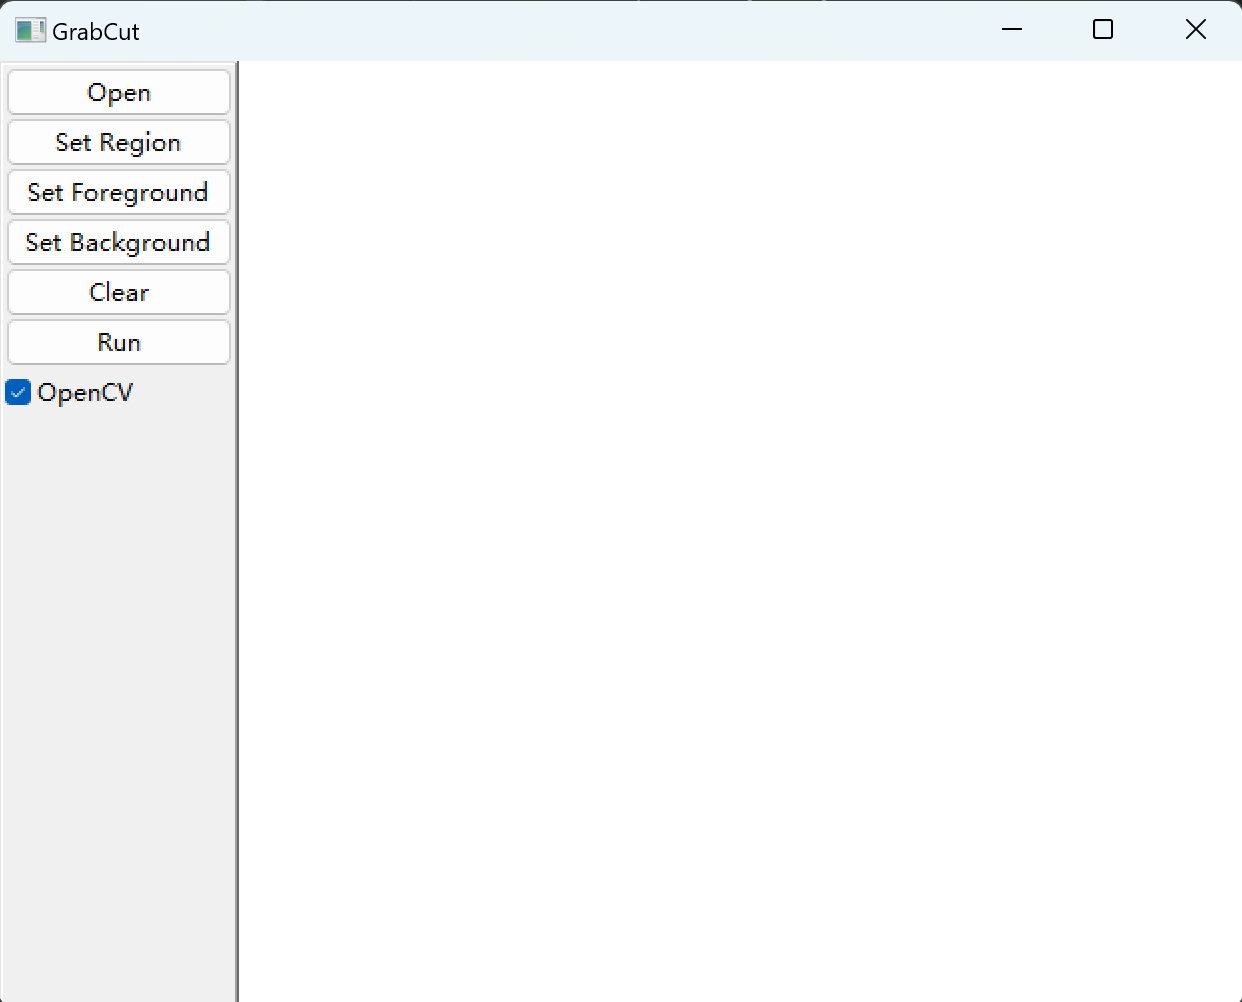
\includegraphics[width=0.49\textwidth]{Initial_page.png}
    \caption{交互页面}
\end{figure}
程序的运行结果图如下:\\
\begin{figure}[H]
	\centering
	\begin{minipage}{0.49\linewidth}
		\centering
		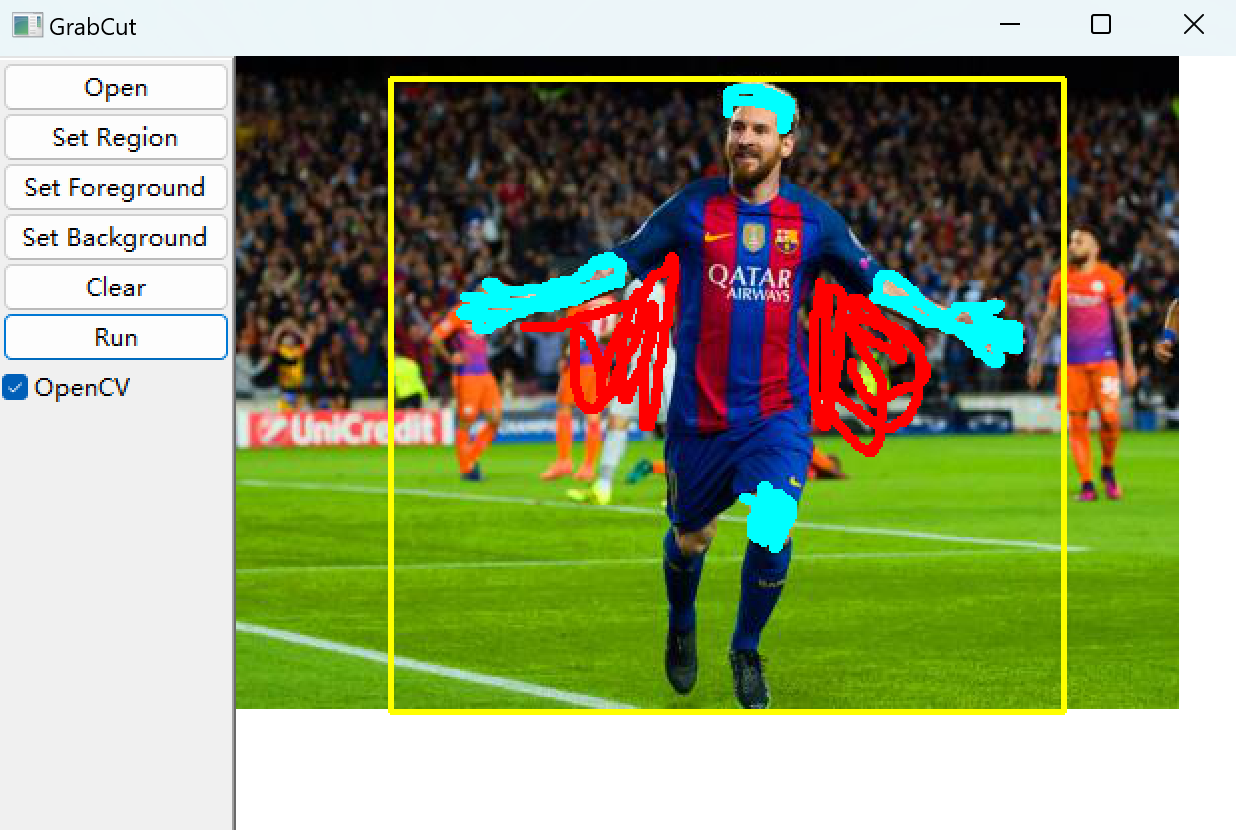
\includegraphics[width=0.9\linewidth]{P1.png}
		\caption{操作图}
		\label{g1}%文中引用该图片代号
	\end{minipage}
	\begin{minipage}{0.49\linewidth}
		\centering
		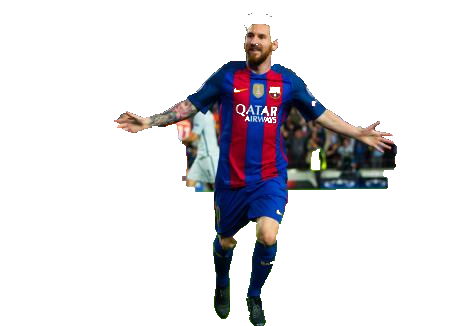
\includegraphics[width=0.9\linewidth]{P1_2.png}
		\caption{结果1}
		\label{g2}%文中引用该图片代号
	\end{minipage}
	%\qquad
	%让图片换行,
	
	\begin{minipage}{0.49\linewidth}
		\centering
		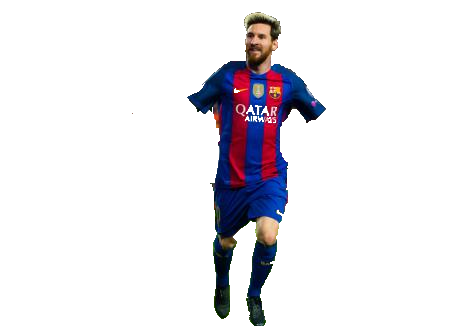
\includegraphics[width=0.9\linewidth]{P1_21.png}
		\caption{结果2}
		\label{g3}%文中引用该图片代号
	\end{minipage}
	\begin{minipage}{0.49\linewidth}
		\centering
		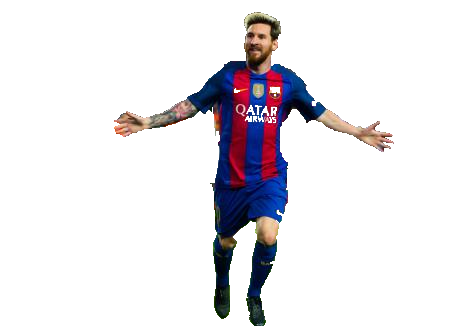
\includegraphics[width=0.9\linewidth]{P1_22.png}
		\caption{结果3}
		\label{g4}%文中引用该图片代号
	\end{minipage}
\end{figure}
可以看到,在第一次直接画矩形框得到的结果(如图\ref{g2})中,梅西的头发没有被检测为前景
且手臂下方的部分区域被误判为前景。此时手动标记被误判的前景和背景(蓝色画笔表示该区域
为前景,红色画笔表示该区域为背景),得到第二次的结果图(如图\ref{g3}),这时梅西的手臂“没了”,
再手动标记梅西的手臂作为前景得到最后的结果(如图\ref{g4});可以看到最后的结果效果比较好。\\
\begin{figure}[H]
	\centering
	\begin{minipage}{0.3\linewidth}
		\centering
		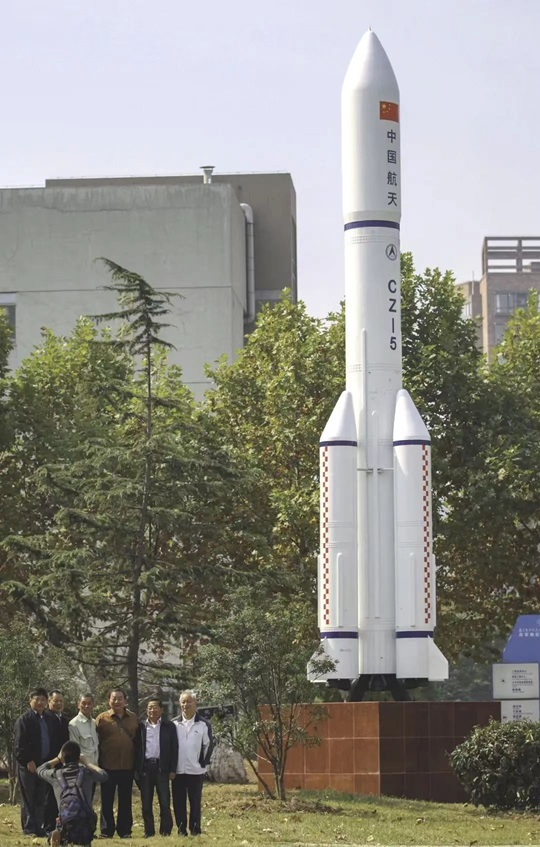
\includegraphics[width=0.9\linewidth]{P2.jpg}
		\caption{原图}
		\label{f1}%文中引用该图片代号
	\end{minipage}
	\begin{minipage}{0.3\linewidth}
		\centering
		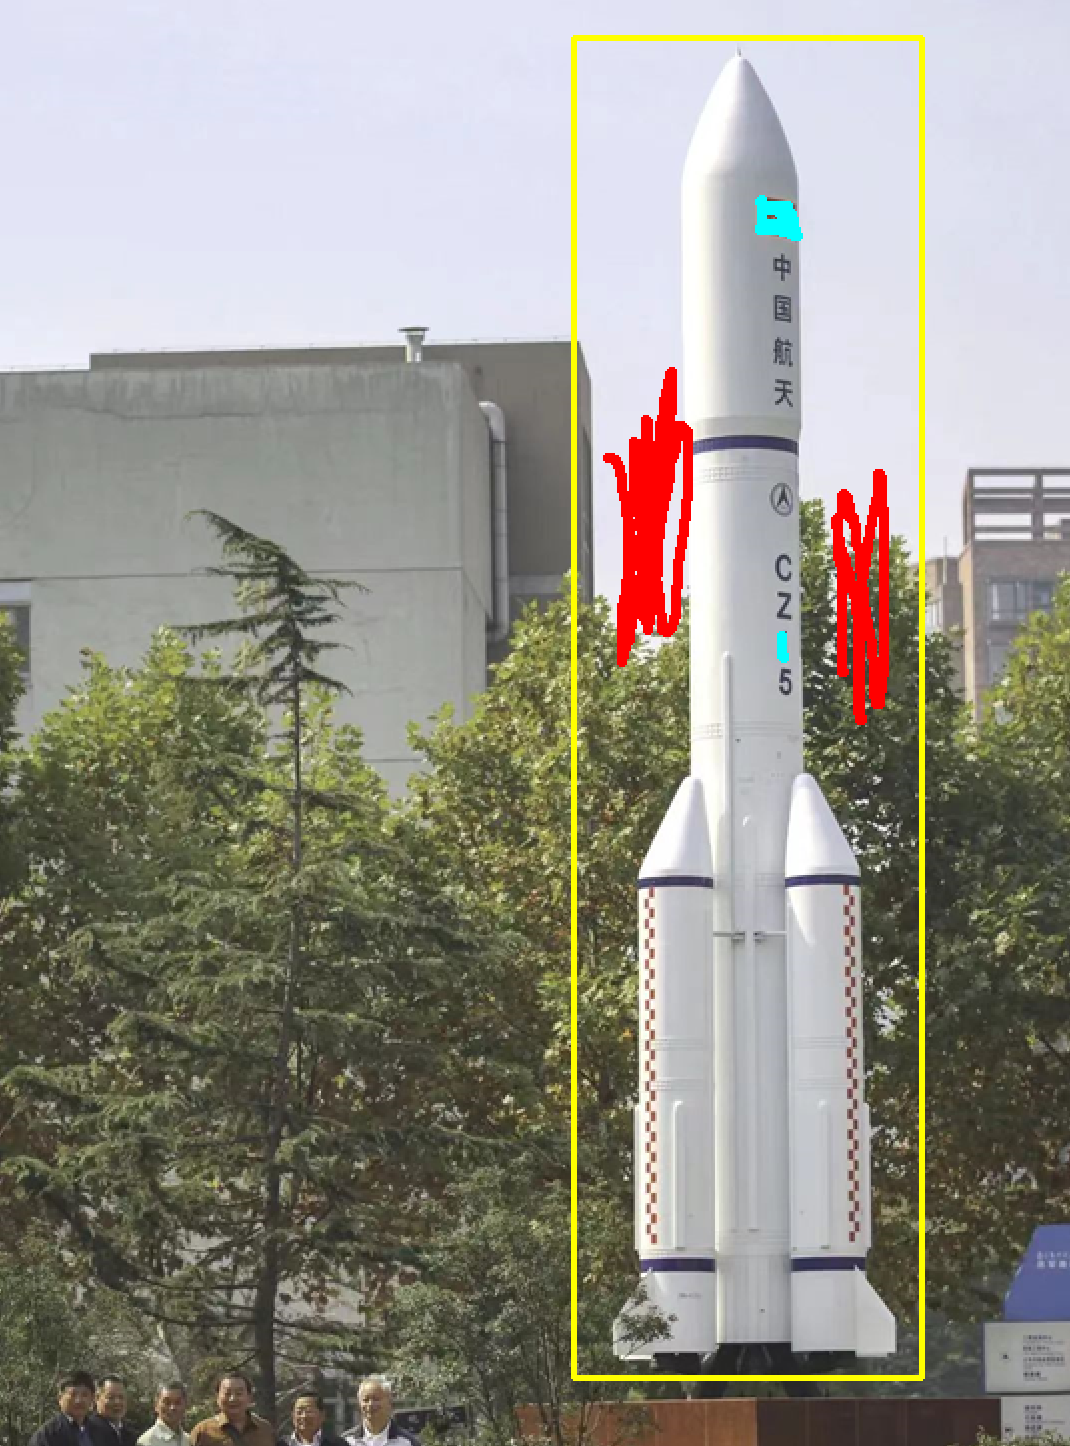
\includegraphics[width=0.9\linewidth]{P2.png}
		\caption{操作图}
		\label{f2}%文中引用该图片代号
	\end{minipage}
	%\qquad
	%让图片换行,
	
	\begin{minipage}{0.3\linewidth}
		\centering
		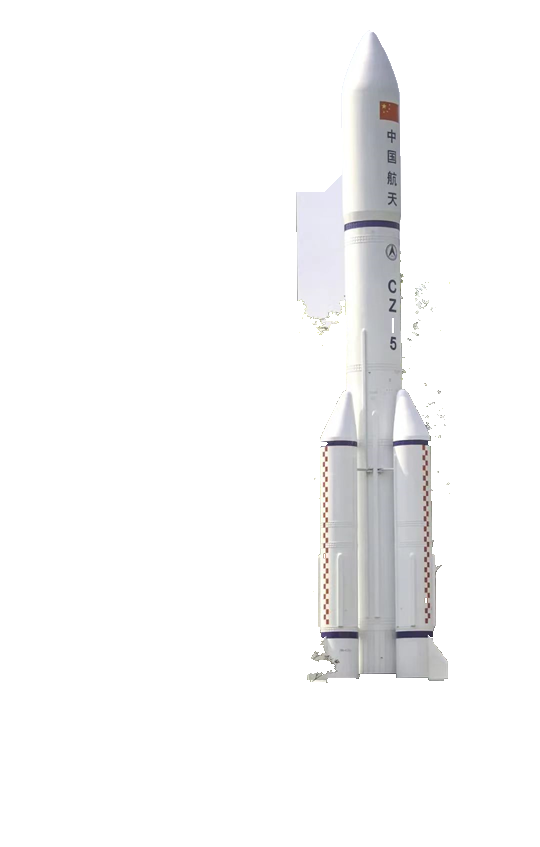
\includegraphics[width=0.9\linewidth]{P2_1}
		\caption{结果1}
		\label{f3}%文中引用该图片代号
	\end{minipage}
	\begin{minipage}{0.3\linewidth}
		\centering
		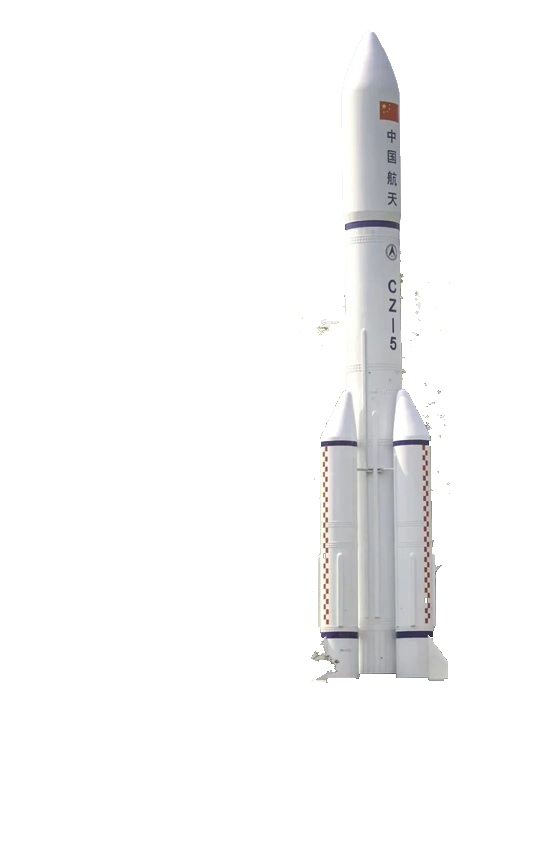
\includegraphics[width=0.9\linewidth]{out.png}
		\caption{结果2}
		\label{f4}%文中引用该图片代号
	\end{minipage}
\end{figure}
此次操作的结果和流程同上。

\subsection{实验结果分析}
由实验结果可知, GrabCut 算法的实验效果很好,具有以下优势:
\begin{itemize}
    \item \textbf{自动化程度高}:只需要用户提供少量初始标记,算法能自动完成大部分分割工作。
    \item \textbf{精确性高}:利用 GMM 和图割,可以在颜色分布和像素连接性上实现精确分割。
    \item \textbf{交互性好}:用户可以随时通过新增标记来修正分割结果。
\end{itemize}
虽然 GrabCut 算法在图像分割中表现出色,但它也存在一些不足和待改进之处。\newline
\textbf{1.处理复杂背景的能力有限}\newline
当前景和背景的颜色分布相似或背景复杂时, GMM 可能难以有效区分前景和背景。
类似颜色的区域可能会被误分类,从而影响分割精度。\\
\textbf{2.计算复杂度高}\newline
迭代优化过程中需要反复训练 GMM 并进行图割,计算复杂度较高,
处理大规模图像时可能会导致计算时间过长。本程序在笔记本上实际消耗的平均时间为4.6秒左右。\\
\textbf{3.对局部细节处理不足}\newline
GrabCut 算法在处理局部细节和小物体时可能表现不佳,尤其是当前景和背景之间的边界复杂时,
可能会出现过度平滑或细节丢失的问题。\\
\textbf{4.依赖用户标记}\newline
GrabCut 算法需要用户提供初始标记(通常是一个矩形框)来区分前景和背景。对于复杂的图像或
用户不确定前景和背景边界的情况,这种依赖可能会导致不准确的初始分割,从而影响最终结果。\\
针对以上问题,可能的改进方向有:\\
\textbf{1.增强GMM建模}\newline
为了解决前景和背景颜色分布相似的问题,可以使用更复杂的建模方法。例如,使用混合模型或
条件随机场(CRF)来替代 GMM ,以更精确地描述像素间的关系。\\
\textbf{2.加速算法}\newline
可以通过并行计算或优化算法(如快速图割算法)来提高计算效率。
有条件的话,使用GPU加速GMM训练和图割优化过程,能够显著减少计算时间。\\
\textbf{3.集成深度学习方法}\newline
将GrabCut与深度学习方法结合,利用深度学习模型提取高级特征,提高分割精度。
可以训练一个端到端的深度学习网络,该网络结合了GrabCut的思想,
通过监督学习自动进行前景和背景分割。
\textbf{4.多尺度处理}\newline
引入多尺度处理方法,通过在不同尺度上进行分割,并融合多尺度信息,
能够更好地处理局部细节和小物体分割问题。这种方法可以减少过度平滑和细节丢失的问题。\\
\textbf{5.用户交互改进}\newline
提供更丰富的用户交互方式,如笔刷标记、擦除工具等,允许用户更加精细地标记前景和背景区域。
通过实时反馈用户操作的分割结果,提高用户体验和分割精度。


\subsection{结论与总结}
GrabCut 算法在图像分割中发挥了重要作用,其创新性的结合GMM和图割技术,结合了用户交互和自动优化,
既保证了分割结果的准确性,又提高了算法的鲁棒性,为图像处理和计算机视觉领域
提供了强有力的工具。通过不断的改进和优化, GrabCut 算法有望在未来的应用中表现得更加出色,
为图像分割技术的发展做出更大的贡献。

\section{心得体会}
在学习了“计算机视觉”课程之后,我们对这一领域有了更加全面和深入的理解,并在实验课上积累了一定的实践经验。

计算机视觉是一个高度实践性的领域。在学习过程中,我们发现理论知识与实际应用密不可分。通过学习基础理论,
如图像处理、特征提取、模式识别等,我们理解了计算机视觉的基本原理。在实验课中,通过编写代码和进行实验,
亲身体验了这些理论在实际问题中的应用。理论与实践相结合的学习方式,使我们对知识的掌握更加牢固,也更能解决实际问题。

在做大作业的时候也发现,计算机视觉是一个快速发展的领域,新技术、新算法层出不穷。我们意识到保持持续学习和创新的能力至关重要。
通过阅读最新的研究论文,我们不仅了解了前沿的发展动态,也激发了自己的创新思维。在实验课中,
我们不断尝试新方法、新技术,提升了创新能力。

最后,感谢老师的悉心教导和同学们的热心帮助,使我们在这段学习旅程中收获颇丰。希望在未来的学习和工作中,
能够将所学知识应用到实际中,为计算机视觉的发展贡献自己的力量。

\section{参考文献}
\begin{thebibliography}{9}
    
    \bibitem{GrabCut}
    C. Rother, V. Kolmogorov, and A. Blake, ""GrabCut": Interactive foreground extraction using iterated graph cuts," \textit{ACM Transactions on Graphics (TOG)}, vol. 23, no. 3, pp. 309-314, 2004.
    
    \bibitem{GraphCuts}
    Y. Boykov and M. P. Jolly, "Interactive graph cuts for optimal boundary \& region segmentation of objects in ND images," \textit{Proceedings of the Eighth IEEE International Conference on Computer Vision (ICCV 2001)}, vol. 1, pp. 105-112, 2001.
    
    \bibitem{DeepGrabCut}
    N. Xu, B. Price, S. Cohen, and T. S. Huang, "Deep GrabCut for object selection," \textit{BMVC}, 2017.
    
    \bibitem{GraphCutsOptimization}
    X. Wang and X. Bai, "Graph Cuts Optimization for Object-based Image Segmentation," \textit{IEEE Transactions on Image Processing}, vol. 26, no. 5, pp. 2474-2489, 2017.
    \end{thebibliography}
\end{sloppypar}
\end{CJK}
\end{document}